\documentclass[a4paper]{report}
% Some basic packages
\usepackage[utf8]{inputenc}
\usepackage[T1]{fontenc}
\usepackage{textcomp}
\usepackage[english]{babel}
\usepackage{url}
\usepackage{graphicx}
\usepackage{float}
\usepackage{booktabs}
\usepackage{enumitem}

\pdfminorversion=7

% Don't indent paragraphs, leave some space between them
\usepackage{parskip}

% Hide page number when page is empty
\usepackage{emptypage}
\usepackage{subcaption}
\usepackage{multicol}
\usepackage{xcolor}

% Other font I sometimes use.
% \usepackage{cmbright}

% Math stuff
\usepackage{amsmath, amsfonts, mathtools, amsthm, amssymb}
% Fancy script capitals
\usepackage{mathrsfs}
\usepackage{cancel}
% Bold math
\usepackage{bm}
% Some shortcuts
\newcommand\N{\ensuremath{\mathbb{N}}}
\newcommand\R{\ensuremath{\mathbb{R}}}
\newcommand\Z{\ensuremath{\mathbb{Z}}}
\renewcommand\O{\ensuremath{\emptyset}}
\newcommand\Q{\ensuremath{\mathbb{Q}}}
\newcommand\C{\ensuremath{\mathbb{C}}}
\renewcommand\L{\ensuremath{\mathcal{L}}}

% Package for Petri Net drawing
\usepackage[version=0.96]{pgf}
\usepackage{tikz}
\usetikzlibrary{arrows,shapes,automata,petri}
\usepackage{tikzit}
\input{petri_nets_style.tikzstyles}

% Easily typeset systems of equations (French package)
\usepackage{systeme}

% Put x \to \infty below \lim
\let\svlim\lim\def\lim{\svlim\limits}

%Make implies and impliedby shorter
\let\implies\Rightarrow
\let\impliedby\Leftarrow
\let\iff\Leftrightarrow
\let\epsilon\varepsilon

% Add \contra symbol to denote contradiction
\usepackage{stmaryrd} % for \lightning
\newcommand\contra{\scalebox{1.5}{$\lightning$}}

% \let\phi\varphi

% Command for short corrections
% Usage: 1+1=\correct{3}{2}

\definecolor{correct}{HTML}{009900}
\newcommand\correct[2]{\ensuremath{\:}{\color{red}{#1}}\ensuremath{\to }{\color{correct}{#2}}\ensuremath{\:}}
\newcommand\green[1]{{\color{correct}{#1}}}

% horizontal rule
\newcommand\hr{
    \noindent\rule[0.5ex]{\linewidth}{0.5pt}
}

% hide parts
\newcommand\hide[1]{}

% si unitx
\usepackage{siunitx}
\sisetup{locale = FR}

% Environments
\makeatother
% For box around Definition, Theorem, \ldots
\usepackage{mdframed}
\mdfsetup{skipabove=1em,skipbelow=0em}
\theoremstyle{definition}
\newmdtheoremenv[nobreak=true]{definitie}{Definitie}
\newmdtheoremenv[nobreak=true]{eigenschap}{Eigenschap}
\newmdtheoremenv[nobreak=true]{gevolg}{Gevolg}
\newmdtheoremenv[nobreak=true]{lemma}{Lemma}
\newmdtheoremenv[nobreak=true]{propositie}{Propositie}
\newmdtheoremenv[nobreak=true]{stelling}{Stelling}
\newmdtheoremenv[nobreak=true]{wet}{Wet}
\newmdtheoremenv[nobreak=true]{postulaat}{Postulaat}
\newmdtheoremenv{conclusie}{Conclusie}
\newmdtheoremenv{toemaatje}{Toemaatje}
\newmdtheoremenv{vermoeden}{Vermoeden}
\newtheorem*{herhaling}{Herhaling}
\newtheorem*{intermezzo}{Intermezzo}
\newtheorem*{notatie}{Notatie}
\newtheorem*{observatie}{Observatie}
\newtheorem*{exe}{Exercise}
\newtheorem*{opmerking}{Opmerking}
\newtheorem*{praktisch}{Praktisch}
\newtheorem*{probleem}{Probleem}
\newtheorem*{terminologie}{Terminologie}
\newtheorem*{toepassing}{Toepassing}
\newtheorem*{uovt}{UOVT}
\newtheorem*{vb}{Voorbeeld}
\newtheorem*{vraag}{Vraag}

\newmdtheoremenv[nobreak=true]{definition}{Definition}
\newtheorem*{eg}{Example}
\newtheorem*{notation}{Notation}
\newtheorem*{previouslyseen}{As previously seen}
\newtheorem*{remark}{Remark}
\newtheorem*{note}{Note}
\newtheorem*{problem}{Problem}
\newtheorem*{observe}{Observe}
\newtheorem*{property}{Property}
\newtheorem*{intuition}{Intuition}
\newmdtheoremenv[nobreak=true]{prop}{Proposition}
\newmdtheoremenv[nobreak=true]{theorem}{Theorem}
\newmdtheoremenv[nobreak=true]{corollary}{Corollary}

% End example and intermezzo environments with a small diamond (just like proof
% environments end with a small square)
\usepackage{etoolbox}
\AtEndEnvironment{vb}{\null\hfill$\diamond$}%
\AtEndEnvironment{intermezzo}{\null\hfill$\diamond$}%
% \AtEndEnvironment{opmerking}{\null\hfill$\diamond$}%

% Fix some spacing
% http://tex.stackexchange.com/questions/22119/how-can-i-change-the-spacing-before-theorems-with-amsthm
\makeatletter
\def\thm@space@setup{%
  \thm@preskip=\parskip \thm@postskip=0pt
}


% Exercise 
% Usage:
% \exercise{5}
% \subexercise{1}
% \subexercise{2}
% \subexercise{3}
% gives
% Exercise 5
%   Exercise 5.1
%   Exercise 5.2
%   Exercise 5.3
\newcommand{\exercise}[1]{%
    \def\@exercise{#1}%
    \subsection*{Exercise #1}
}

\newcommand{\subexercise}[1]{%
    \subsubsection*{Exercise \@exercise.#1}
}


% \lecture starts a new lecture (les in dutch)
%
% Usage:
% \lecture{1}{di 12 feb 2019 16:00}{Inleiding}
%
% This adds a section heading with the number / title of the lecture and a
% margin paragraph with the date.

% I use \dateparts here to hide the year (2019). This way, I can easily parse
% the date of each lecture unambiguously while still having a human-friendly
% short format printed to the pdf.

\usepackage{xifthen}
\def\testdateparts#1{\dateparts#1\relax}
\def\dateparts#1 #2 #3 #4 #5\relax{
    \marginpar{\small\textsf{\mbox{#1 #2 #3 #5}}}
}

\def\@lecture{}%
\newcommand{\lecture}[3]{
    \ifthenelse{\isempty{#3}}{%
        \def\@lecture{Lecture #1}%
    }{%
        \def\@lecture{Lecture #1: #3}%
    }%
    \subsection*{\@lecture}
    \marginpar{\small\textsf{\mbox{#2}}}
}



% These are the fancy headers
\usepackage{fancyhdr}
\pagestyle{fancy}

% LE: left even
% RO: right odd
% CE, CO: center even, center odd
% My name for when I print my lecture notes to use for an open book exam.
% \fancyhead[LE,RO]{Gilles Castel}

\fancyhead[RO,LE]{\@lecture} % Right odd,  Left even
\fancyhead[RE,LO]{}          % Right even, Left odd

\fancyfoot[RO,LE]{\thepage}  % Right odd,  Left even
\fancyfoot[RE,LO]{}          % Right even, Left odd
\fancyfoot[C]{\leftmark}     % Center

\makeatother




% Todonotes and inline notes in fancy boxes
\usepackage{todonotes}
\usepackage{tcolorbox}

% Make boxes breakable
\tcbuselibrary{breakable}

% Verbetering is correction in Dutch
% Usage: 
% \begin{verbetering}
%     Lorem ipsum dolor sit amet, consetetur sadipscing elitr, sed diam nonumy eirmod
%     tempor invidunt ut labore et dolore magna aliquyam erat, sed diam voluptua. At
%     vero eos et accusam et justo duo dolores et ea rebum. Stet clita kasd gubergren,
%     no sea takimata sanctus est Lorem ipsum dolor sit amet.
% \end{verbetering}
\newenvironment{verbetering}{\begin{tcolorbox}[
    arc=0mm,
    colback=white,
    colframe=green!60!black,
    title=Opmerking,
    fonttitle=\sffamily,
    breakable
]}{\end{tcolorbox}}

% Noot is note in Dutch. Same as 'verbetering' but color of box is different
\newenvironment{noot}[1]{\begin{tcolorbox}[
    arc=0mm,
    colback=white,
    colframe=white!60!black,
    title=#1,
    fonttitle=\sffamily,
    breakable
]}{\end{tcolorbox}}




% Figure support as explained in my blog post.
\usepackage{import}
\usepackage{xifthen}
\usepackage{pdfpages}
\usepackage{transparent}
\newcommand{\incfig}[1]{%
    \def\svgwidth{\columnwidth}
    \import{./figures/}{#1.pdf_tex}
}

% Fix some stuff
% %http://tex.stackexchange.com/questions/76273/multiple-pdfs-with-page-group-included-in-a-single-page-warning
\pdfsuppresswarningpagegroup=1


% My name
\author{Bruno M. Pacheco}

 
\begin{document}
 
\title{Laboratório 7}
\author{Bruno M. Pacheco (16100865)\\
Pedro Y. F. Ceripes (18100681) \\
EEL 7550 - Eletrônica Aplicada}

\maketitle
\section*{Objetivo}

As experiências relatadas neste documento visam demonstrar e garantir experiência nos diversos arranjos para polarização de transistores de junção bipolar, manipulando os valores dos resistores utilizados para atingir um dado ponto de operação.

\section*{Simulações}

\subsection*{Circuito 1}
\subsection*{a}

Escolhendo o ponto de operação de $\mathbf{I_C = 2mA}$ e $\mathbf{V_{CE} = 4V}$, e observando que $V_{BE}=660mV$ e $\beta = 290$ típicos fornecidos pelo fabricante, e conhecendo a relação:
\begin{equation}
        I_C = \beta \frac{V_{cc}-V_{BE}}{R_B};
\end{equation}
\begin{equation} 
        V_{CE} = V_{cc} - I_C R_C.
\end{equation}
    
Podemos calcular o valor de $R_B$ como sendo,
\begin{equation*}
    R_B = \beta \frac{V_{cc}-V_{BE}}{I_C} = 1.64 M \Omega.
\end{equation*}

Além disso, podemos calcular $R_C$, como:
\begin{equation*}
    R_C = \frac{V_{cc}-V_{CE}}{I_C} = 4k\Omega.
\end{equation*}

\subsection*{b}
Com base na tabela de valores comerciais de resistores podemos escolher os resistores de $R_B = 1.6M \Omega$ e  $R_C = 4.3k \Omega$. A partir disso, e utilizando os valores  $\beta_{min} = 200 $ e $\beta_{max} = 450$ , obtemos os resultados.
\begin{table}[!h]
    \centering
    \begin{tabular}{|c|c|c|c|}
    \hline
    $I_C(\beta_{min})$	&	$I_C(\beta_{max})$	&	$V_{CE}(\beta_{min})$	&	$V_{CE}(\beta_{max})$	\\	\hline
1.42mA	&	3.19mA	&	5.91V	&	-1.71V	\\	\hline
    \end{tabular}
    \caption{$I_C$ e $V_{BE}$ os limites do $\beta$.}
    \label{tab:Q1}
\end{table}

\subsection*{c}

Para realizar a simulação, foi montado o circuito abaixo:

\begin{figure}[H]
    \centering
    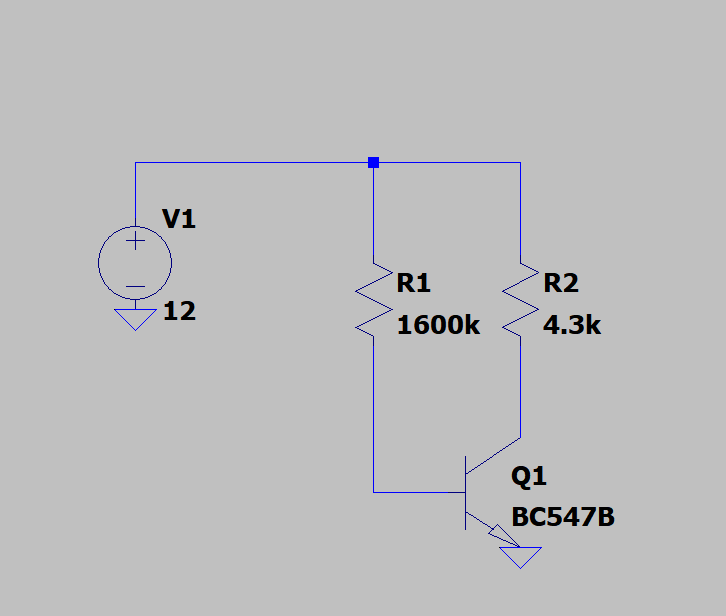
\includegraphics[width=0.8\textwidth]{figures/lab7-1-c.png}
    \caption{Primeiro circuito configurado no LTSpice.}
    \label{fig:figures-lab7-1-c-png}
\end{figure}

Simulando o circuito da figura, obtemos as seguintes medições.
\begin{table}[!h]
    \centering
    \begin{tabular}{|c|c|c|}
\hline
$\beta$	&	$I_C$	&	$V_{CE}$	\\	\hline
291.72	&	2.068mA	&	3.1075V	\\	\hline

    \end{tabular}
    \caption{Parâmetros simulados }
    \label{tab:Q1c}
\end{table}
\subsection*{Circuito 2}

\subsection*{a}

Escolhendo o ponte de operação $\mathbf{I_C = 2mA}$ e $\mathbf{V_{CE} = 4V}$ com $\mathbf{R_B = 1M \Omega}$, $\mathbf{R_C = 1.8k\Omega}$ e $\mathbf{R_E = 2.2 k \Omega}$ e conhecendo a relação:


\begin{equation}
        I_C = \beta \frac{V_{cc}-V_{BE}}{R_B+ (1+\beta)R_E},
\end{equation}
\begin{equation} 
        V_{CE} = V_{cc} - I_C (R_C + R_E).
\end{equation}



Podemos utilizar os mesmos valores limites de $\beta$ para completar a tabela abaixo:
\begin{table}[H]
    \centering
    \begin{tabular}{|c|c|c|c|}
    \hline
    $I_C(\beta_{min})$	&	$I_C(\beta_{max})$	&	$V_{CE}(\beta_{min})$	&	$V_{CE}(\beta_{max})$	\\	\hline
1.57mA	&	2.56mA	&	5.71V	&	1.75V	\\	\hline

    \end{tabular}
    \caption{$I_C$ e $V_{BE}$ calculados para os limites de $\beta$.}
    \label{tab:Q2a}
\end{table}
\subsection*{b}

Para realizar a simulação, foi montado o circuito abaixo:

\begin{figure}[H]
    \centering
    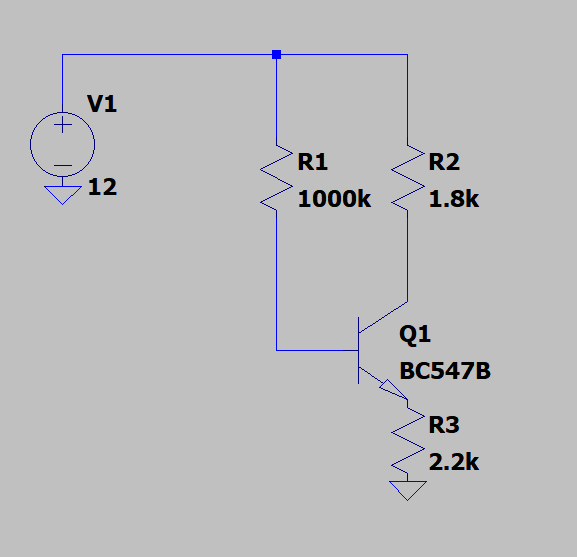
\includegraphics[width=0.8\textwidth]{figures/lab7-2-b.png}
    \caption{Segundo circuito configurado no LTSpice.}
    \label{fig:figures-lab7-1-c-png}
\end{figure}


Simulando o circuito da figura, obtemos os seguintes valores.

\begin{table}[!h]
    \centering
    \begin{tabular}{|c|c|c|}
        \hline
         $\beta$	&	$I_C$	&	$V_{CE}$	\\	\hline
295.34	&	2.028mA	&	3.8731V	\\	\hline

    \end{tabular}
    \caption{Parâmetros simulados}
    \label{tab:Q2b}
\end{table}

\subsection*{Circuito 3}
\subsection*{a}
Para o ponto de operação semelhante ao do exercício passado, porém utilizando os novos resistores, temos que:
    \begin{equation}
        V_{TH} = \frac{R_2 V_{cc}}{R_1+R_2};
    \end{equation}
    \begin{equation}
        R_{TH} = \frac{R_1 R_2}{R_1+R_2};
    \end{equation}
    \begin{equation}
        I_C =\beta \frac{V_{TH}- V_{BE}}{R_{TH} + (1+\beta)R_E};
    \end{equation}
    \begin{equation}
        V_{CE} = V_{cc} - I_C(R_C + R_E).
    \end{equation}

Calculamos os valores de $\mathbf{I_C} $ e $\mathbf{V_{CE}}$ para os limites de $\beta$, presentes na tabela abaixo.

\begin{table}[!h]
    \centering
    \begin{tabular}{|c|c|c|c|}
    \hline
    $I_C(\beta_{min})$	&	$I_C(\beta_{max})$	&	$V_{CE}(\beta_{min})$	&	$V_{CE}(\beta_{max})$	\\	\hline
2.08mA	&	2.11mA	&	3.67V	&	3.58V	\\	\hline
    \end{tabular}
    \caption{}
    \label{tab:Q3a}
\end{table}

\subsection*{b}


Para realizar a simulação, foi montado o circuito abaixo:

\begin{figure}[H]
    \centering
    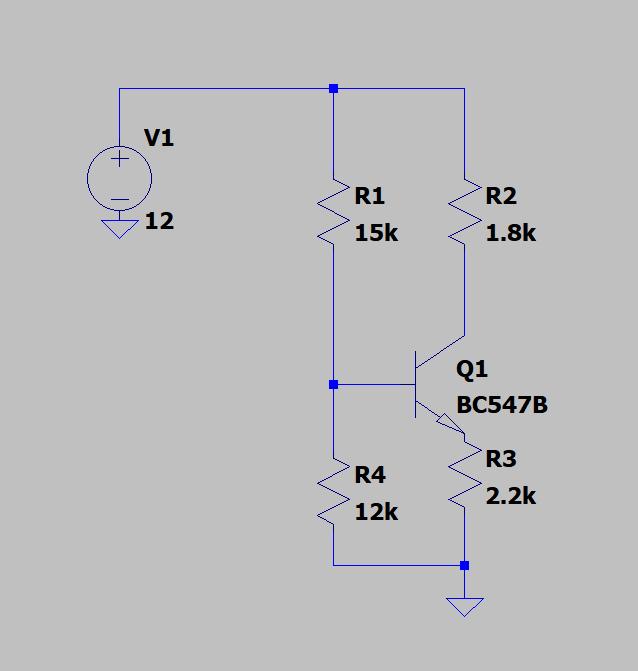
\includegraphics[width=0.8\textwidth]{figures/lab7-3-b.png}
    \caption{Terceiro circuito configurado no LTSpice.}
    \label{fig:figures-lab7-1-c-png}
\end{figure}


Simulando o circuito da figura, obtemos os seguintes valores.

\begin{table}[!h]
    \centering
    \begin{tabular}{|c|c|c|}
    \hline
         $\beta$	&	$I_C$	&	$V_{CE}$	\\	\hline
293.93	&	2.0965mA	&	3.5983V	\\	\hline

    \end{tabular}
    \caption{Parâmetros simulados}
    \label{tab:Q3b}
\end{table}


\section{Conclusão}

Dentre as diversas experiências, foram expostas e testadas as características dos diversos circuitos básicos para polarização de transistores BJT. Dentre eles, foram validadas os diferentes requisitos em termo de arranjo dos componentes para atingir um mesmo ponto de operação, inclusive as variações relativas as não idealidades.

\end{document}
